\section{绘图}
SAC中有四个绘图命令,分别是\nameref{plot}、\nameref{plot1}、\nameref{plot2}、
\nameref{plotpk}。

plotpk用于``人机交互''过程中拾取震相,在\nameref{sec:picking}中会详细讲解。

下面说说plot、plot1和plot2的区别。

当内存中只有一个文件的时候,这三个绘图命令是没有区别的;而当内存中存在
多个文件时,区别就非常明显了。

\subsection{plot}
plot命令会在单个图形窗口中显示单个波形。
\begin{SACCode}
SAC> r cdv.[nez]
SAC> p
Waiting
Waiting
SAC>
\end{SACCode}
将三个波形数据读入内存,使用plot时,焦点位于绘图窗口,且绘图窗口上只显示
第一个波形,且终端中出现``Waiting''字样;将焦点切换\footnote{Alt+Tab}回终端,
键入``Enter'',绘图窗口中显示第二个波形,终端中出现第二个``Waiting''字样,
焦点位于终端中;再次键入``Enter'',窗口中显示第三个波形,焦点位于终端,
由于已经没有更多的波形需要显示,此时终端中显示SAC提示符。

如果内存中还有波形在``Waiting'',而你想要退出plot,不想要再继续查看后面的波形,
可以在终端中键入``kill''(简写为k),以直接退出plot。
\begin{SACCode}
SAC> r cdv.[nez]
SAC> p
Waitingk
SAC>
\end{SACCode}

\subsection{plot1}
plot1命令会在一个窗口中显示多个波形。波形会共用一个X轴,且具有单独的Y轴。
\begin{SACCode}
SAC> r cdv.?
cdv.e cdv.n cdv.z
SAC> p1
\end{SACCode}
执行plot1命令后,焦点位于图形窗口,显示如图\ref{fig:plot1}。
\begin{figure}[H]
\centering
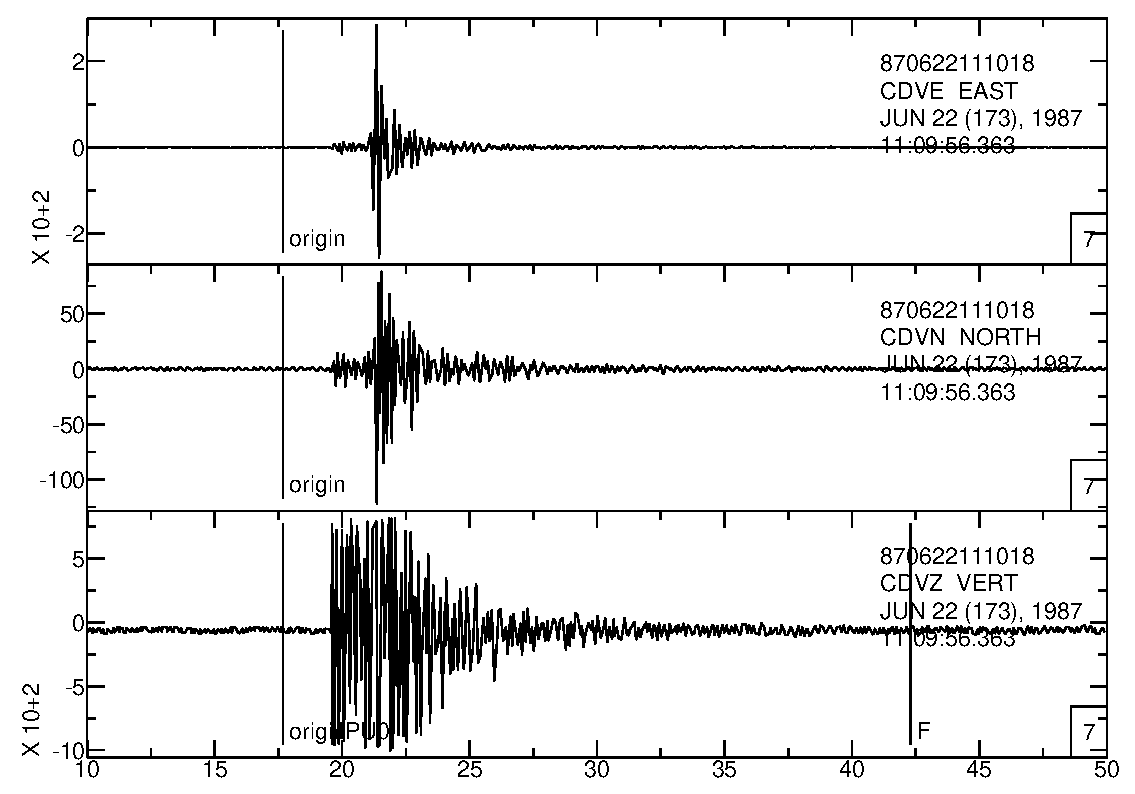
\includegraphics[width=\textwidth]{plot1}
\caption{plot1绘图效果}
\label{fig:plot1}
\end{figure}

当一次性读入很多个地震数据时,如果直接使用plot1绘图,会导致一个窗口内有太多
波形,反而什么都看不清,plot1提供了额外的选项和参数以指定一个窗口内的最大
波形数,多余的波形则处于等待状态。
\begin{SACCode}
SAC> dg sub local cdv.[enz] cvl.[enz] cvy.[enz]
cdv.e cdv.n cdv.z cvl.e cvl.n cvl.z cvy.e cvy.n cvy.z
SAC> p1 p 3         // p是选项perplot的简写,3代表每次3个波形
Waiting
Waiting
SAC> 
\end{SACCode}
经常遇到的情况是,想要将每个台站的三个分量放在一起看,这个时候设置选项perplot的参数值为3即可。

\subsection{plot2}
plot2会在一个窗口内绘制多个波形,波形共用X轴和Y轴。
\begin{SACCode}
SAC> fg seis                     // 生成数据
SAC> rmean; rtrend; taper        // 预处理
SAC> w seis.0                    // 写入滤波前文件
SAC> bp c 0.05 10 n 4 p 2        // 滤波
SAC> w seis.1                    // 写入滤波后文件
SAC> r ./seis.[01]               // 读入两个文件
./seis.0 ...seis.1
SAC> color red inc list red blue // 设置颜色
SAC> p2                          // 绘图
\end{SACCode}
绘图效果如图\ref{fig:plot2},显然plot2比较适合在对比波形时使用。

\begin{figure}[H]
\centering
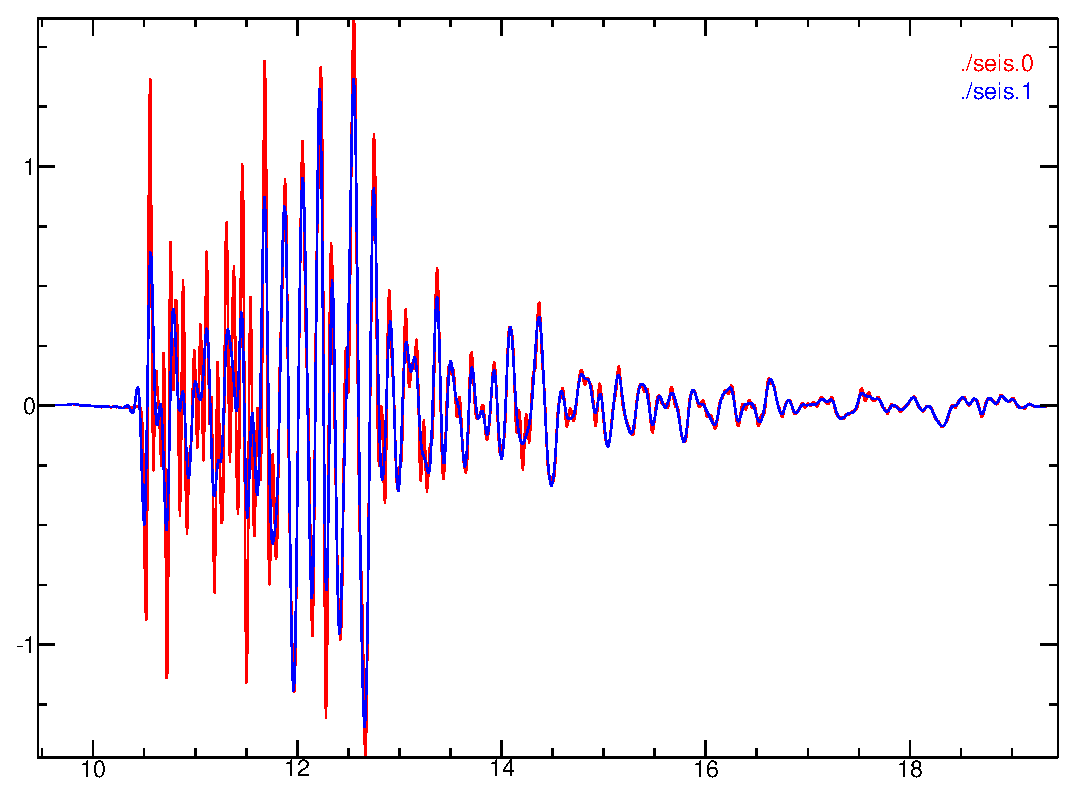
\includegraphics[width=\textwidth]{plot2}
\caption[plot2绘图效果]{plot2绘图效果。红色为滤波前波形,蓝色为滤波后波形。}
\label{fig:plot2}
\end{figure}
